\section{Implementation}\label{s:impl}
\begin{figure*}
    \centering
    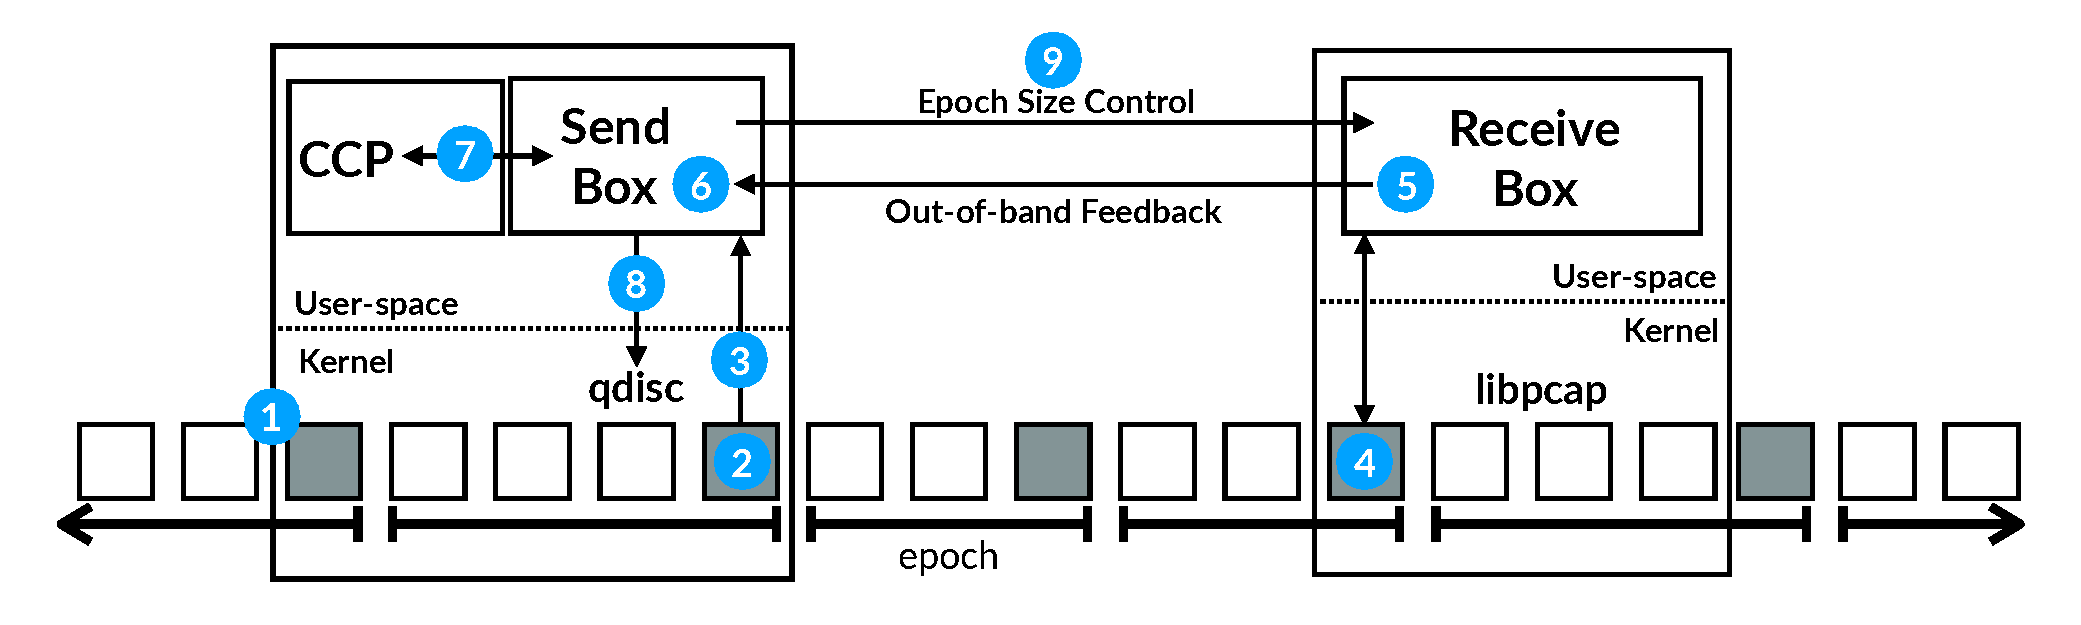
\includegraphics[width=2\columnwidth]{img/bundler-diagram}
    \caption{\name System Design}\label{fig:bundler}
\end{figure*}

The prevalence of middleboxes today means that there are multiple options for implementing a \name.
We envision a two-part design for the \inbox: a ``control-plane'' and ``data-plane'' separation.
The data plane is responsible for packet forwarding, maintaining a count of the in-bundle bytes sent, enforcing a rate and scheduling policy on the bundle, and reporting epoch packets to the control plane.
These operations can be implemented either in software, via modern platforms for network function virtualization~\cite{bess, click, mos, netbricks}, or in hardware via programmable switches~\cite{p4}.
The \outbox is simple and does not require a control plane; it simply must observe the packet stream, maintain a byte count, and send reports to the \inbox on observing epoch packets.
The \outbox can, therefore, be implemented entirely in hardware if necessary.

\subsection{Prototype}\label{s:impl:prototype}
To highlight the simplicity of our approach\footnote{and because we are lazy programmers}, we implement the inbox dataplane using Linux \texttt{tc}~\cite{tc}, and we limit our implementations of scheduling policy to those already widely available in the Linux kernel.
We patch the TBF queueing discipline (qdisc)~\cite{tbf} to enforce rates, and modify its ``inner\_qdisc'' to use a qdisc that enforces some scheduling policy.
Our patch to the TBF qdisc comprises $112$ lines of C.
The patch adds extra logging and the functionality to transmit feedback to the control plane using a netlink socket. 
Additionally, it removes one line in the rate update functionality to disable re-filling the token bucket on rate changes to prevent a penalty for frequent rate updates.

We implement the \inbox control plane to run in user-space in $1167$ lines of Rust. 
It uses \texttt{libnl} to communicate with the qdisc, and \texttt{libccp}~\cite{ccp} to communicate with the congestion control algorithm via Unix-domain sockets.
We use existing implementations of congestion control algorithms on CCP without modification\footnote{We discovered and patched a minor bug in the CCP Copa~\cite{copa} implementation.}; since CCP algorithms are already designed to receive network feedback asynchronously, they are a natural choice for our epoch-based measurement architecture.
It maintains the congestion control state of each bundle, but does not maintain (or observe) per-flow state.

We implement the \outbox using \texttt{libpcap} in $188$ lines of Rust. It listens for packets on the interface, checks for epoch packets, and sends the reports to the \inbox. It must maintain per-bundle counters (described in \S\ref{s:impl:discovery}).

\subsection{\name Event Loop}\label{s:impl:loop}
Figure~\ref{fig:bundler} overviews the operation of our \name implementation.

(1) Packets arriving at the inbox are sent to the qdisc. Those that match a bundle are put into the proper queue, 
otherwise they are forwarded immediately. (2) The qdisc observes one of the packest matches the epoch boundary
condition. (3) It sends a netlink message to the \inbox process running in user-space, which records the packet
in its epoch data structure, then forwards the packet along. (4) The \outbox observes the same epoch boundary
packet. (5) It sends an out-of-band UDP message to the \inbox containing the hash of the packet and its current state. 
(6) The \inbox receives the UDP message, and uses it to calculate the epochs and measurements as described 
in \S\ref{s:measurement}.

(7) Asynchronously, the \inbox invokes the congestion control algorithm every $10$ms via \texttt{libccp},
giving it a chance to observe any new measurements and change its behavior. (8) If it decides to update
the bundle rate or congestion window, the \inbox communicates this to the qdisc
using \texttt{libnl}. Since the qdisc only supports rate enforcement, if the algorithm
also uses a congestion window, the \inbox computes $\text{\emph{effective rate}} = \frac{\text{CWND}}{\text{RTT}}$
and sets the rate of the qdisc to the minimum of the explicit rate and this effective rate.
Upon receiving new RTT samples, the \inbox updates the effective rate, and updates the qdisc rate
if appropriate.

\subsection{Bundle Initialization}\label{s:impl:discovery}

One practical concern in a \name deployment is how the \inbox and \outbox discover each others' presence. Of course, it is always possible to statically configure an \inbox and \outbox; however, this may be impractical as they reside in different networks.
Rather, we propose a bootstrapping mechanism wherein aggregates are formed naturally.
This mechanism classifies packets traversing the \inbox and \outbox as either non-bundled (should be transmitted immediately and not paced in the qdisc) or bundled in a given qdisc. Different bundles may have different rates; recent work~\cite{carousel, eifel} has shown it is possible to implement such multi-rate, multi-scheduler datapaths efficiently.

The \inbox first assumes that all packets which traverse it are not bundled.
The \outbox does one of two things for each potential epoch boundary packet:
\begin{enumerate}
    \item If the packet is in a known bundle, the \outbox sends a message to the corresponding \inbox.
    \item If the packet is not in a known bundle, the \outbox sends a message to the source IP address of that packet.
\end{enumerate}

If there is no \inbox on the path, the packet will simply be ignored at its destination. 
The \inbox receives (and intercepts) the \outbox feedback.  
The \inbox at this time updates its flow tables to add the destination IP of the epoch boundary packet either to an existing bundle (in the case of a new flow from a previously-unseen source subnet joining a bundle) or instantiates a new bundle.
The \inbox then sends a response containing an epoch size to use and the hash of the epoch boundary packet.
The \outbox receives this message, initializes a byte counter for the newly discovered bundle, and remembers the \inbox IP address for future feedback.
